%% ===================================================================
%% An Area-Efficient Pipelined Signed Radix-4 MRPM for Biomedical
%% FIR Filtering -- IEEE Conference format (IEEEtran)
%%
%% STATUS: complete draft. All hardware numbers are MEASURED from Gowin
%% POST-PLACE-AND-ROUTE utilisation/timing/power reports (GW1NR-9C, DSP=0).
%% The design was NOT downloaded to a board; no on-chip execution is
%% claimed anywhere. All functional results are from simulation (0 mismatches).
%%
%% REMAINING TODO BEFORE SUBMISSION:
%%   1. Author block: replace placeholder names/affiliations/emails.
%%   2. Figures 1 and 2 are native TikZ (no external files needed).
%%      Optionally add a third: GTKWave waveform (make fir -> fir.vcd),
%%      the analogue of Fig. 5 in the base paper.
%%   3. Verify the base-paper figures quoted in Sec. VI-D against the PDF.
%%
%% The \TBD macro is retained deliberately: if any future edit introduces
%% an unmeasured number, use \TBD rather than a plausible-looking figure.
%% ===================================================================

\documentclass[conference]{IEEEtran}

\usepackage{cite}
\usepackage{amsmath,amssymb,amsfonts}
\usepackage{algorithmic}
\usepackage{algorithm}
\usepackage{graphicx}
\usepackage{textcomp}
\usepackage{xcolor}
\usepackage{booktabs}
\usepackage{url}
\usepackage{tikz}
\usetikzlibrary{arrows.meta,positioning,calc,fit,backgrounds}

\tikzset{
  blk/.style   = {draw, rectangle, rounded corners=1pt, align=center,
                  font=\scriptsize\sffamily, inner sep=2pt, minimum height=4.2mm},
  smallblk/.style = {draw, rectangle, align=center,
                  font=\tiny\sffamily, inner sep=1.5pt, minimum height=3.4mm},
  reg/.style   = {draw, rectangle, align=center, font=\tiny\sffamily,
                  inner sep=1pt, minimum width=5mm, minimum height=4mm},
  addr/.style  = {draw, circle, font=\tiny\sffamily, inner sep=0.6pt,
                  minimum size=4.2mm},
  io/.style    = {font=\scriptsize\sffamily\bfseries},
  wire/.style  = {-{Latex[length=1.3mm,width=1.1mm]}, line width=0.35pt},
  plain/.style = {line width=0.35pt},
  bw/.style    = {font=\tiny\sffamily, inner sep=0.7pt, fill=white},
  pipe/.style  = {dashed, line width=0.4pt, gray}
}



% Placeholder macro: renders in red so no unmeasured number can slip
% through into a submission unnoticed.
\newcommand{\TBD}{\textcolor{red}{\texttt{[TBD-Gowin]}}}
\newcommand{\VERIFY}{\textcolor{red}{\texttt{[verify vs.~\cite{base}]}}}

\begin{document}

\title{An Area-Efficient Pipelined Signed Radix-4 Modified Russian
Peasant Multiplier for Biomedical FIR Filtering}

\author{
\IEEEauthorblockN{Aditya Garg}
\IEEEauthorblockA{\textit{Dept.\ of Electronics and Communication Engineering} \\
\textit{Institution Name} \\
City, India \\
aditya.garg@email.com}
\and
\IEEEauthorblockN{Ashu Anand}
\IEEEauthorblockA{\textit{Dept.\ of Electronics and Communication Engineering} \\
\textit{Institution Name} \\
City, India \\
ashu.anand@email.com}
}

\maketitle

% ===================================================================
\begin{abstract}
Hardware multipliers dominate the area and power budget of the digital
signal-processing chains used in wearable and implantable biomedical
devices, where silicon area and battery life are tightly constrained.
The Modified Russian Peasant Multiplier (MRPM) has recently been shown
to be an attractive low-area primitive for such systems. This work
extends that architecture in four directions. First, the iterative
unsigned MRPM is replaced by a \emph{signed radix-4 modified-Booth}
formulation that reduces an 8-bit multiplication to four partial
products evaluated in parallel, rather than eight sequential
shift-and-add iterations, while natively supporting two's-complement
operands. Second, the linear-phase symmetry of the filter coefficients
is exploited to \emph{fold} an 8-tap FIR onto four multipliers instead
of eight, reducing LUT4 utilisation of the complete filter from 345 to
222 --- a saving of 35.7\% --- with bit-identical output. Third, the folded datapath is pipelined into four stages,
raising the maximum clock frequency by $1.55\times$ (42.96~MHz to
66.47~MHz). Fourth, four parallel-prefix adder topologies are
synthesised on a common fabric; we find that at 8-bit datapath width
the choice of prefix adder is close to immaterial (222--238 LUT4,
41.8--45.0~MHz), which suggests that effort is better directed at the
partial-product count and the filter structure than at the adder. The
design is exact rather than approximate: the multiplier is verified
exhaustively over all $65{,}536$ signed operand pairs with zero
mismatches, and every filter configuration matches an independent
golden model bit-for-bit. Synthesis and place-and-route for a low-cost Gowin GW1NR-9C FPGA use LUT
logic exclusively, with dedicated DSP inference disabled and zero DSP
blocks confirmed in every run, making the architecture suitable for
area-constrained ECG and EEG front ends.
\end{abstract}

\begin{IEEEkeywords}
Multiplier, Russian Peasant algorithm, Booth recoding, parallel-prefix
adder, parallel-prefix adder, FIR filter, FPGA, biomedical signal
processing, VLSI.
\end{IEEEkeywords}

% ===================================================================
\section{Introduction}
\label{sec:intro}

The design of efficient hardware multipliers remains central to digital
signal processing, because the multiplier is typically the most
area- and power-intensive element of an arithmetic datapath
\cite{sharma,lotfabadi}. This constraint is felt most acutely in
wearable health monitors and implantable biomedical devices, where
every square millimetre of silicon and every microampere of current
directly limits device lifetime and viability \cite{ajay}. Such systems
must simultaneously satisfy three requirements that ordinarily trade
off against one another: computational accuracy, resource efficiency,
and low power.

Classical multiplier architectures --- array, Booth, Wallace-tree and
Vedic designs \cite{phuse,prabhu,gokhale,bansal} --- have been studied
extensively, but their resource utilisation remains high for
resource-constrained deployment. A second family of designs achieves
area and power reduction by \emph{approximating} the product
\cite{khurshid,approx2025}. Approximate multipliers are effective for
error-tolerant workloads such as image processing, but they are
unsuitable for diagnostic biomedical signal chains, where a small
numerical deviation can alter clinical interpretation. An exact,
low-area multiplier is therefore required.

The Russian Peasant Multiplication (RPM) algorithm offers one route to
such a primitive. RPM computes a product by repeatedly halving one
operand and doubling the other, accumulating the doubled operand
whenever the halved operand is odd. Because it reuses a small set of
shift and add resources rather than generating and storing a full
partial-product array, RPM is inherently compact. Recent work by
Subramanian~\textit{et al.}~\cite{base} proposed a Modified Russian
Peasant Multiplier (MRPM) that couples this algorithm with a
Kogge-Stone parallel-prefix adder, and demonstrated its suitability for
biomedical applications on an FPGA platform. That work is the direct
predecessor of the present paper.

Building on \cite{base}, we observe five opportunities for further
optimisation that the base architecture leaves open:

\begin{enumerate}
  \item \textbf{Unsigned operands only.} Biomedical signal processing
  routinely involves differential and mean-removed signals, which are
  inherently signed. An unsigned multiplier requires external sign
  handling, adding logic outside the multiplier boundary.

  \item \textbf{Iteration-bound throughput.} RPM consumes approximately
  one multiplier bit per iteration, requiring on the order of eight
  iterations for an 8-bit operand. Accelerating the \emph{adder} inside
  a sequential loop reduces only the per-iteration cost; the iteration
  count itself remains the dominant term in end-to-end latency.

  \item \textbf{No radix recoding.} The partial-product count is not
  reduced by radix-4 (or higher) recoding, although this is a standard
  and well-understood lever.

  \item \textbf{No structural FIR optimisation.} When the multiplier is
  deployed in an FIR filter, the linear-phase symmetry of the
  coefficient set is not exploited to reduce the multiplier count.

  \item \textbf{Adder choice not swept.} A Kogge-Stone adder is adopted
  without a comparative evaluation against other parallel-prefix
  topologies on the same fabric. Since the depth/cell-count/fan-out
  trade-off among prefix networks is strongly width-dependent, it is not
  self-evident that the minimum-depth topology is the right choice at
  8-bit width.
\end{enumerate}

These are opportunities for extension rather than deficiencies: the base
architecture establishes MRPM as a viable low-area primitive, and this
work asks how much further the same idea can be pushed.

\smallskip\noindent\textbf{Contributions.} This paper makes the
following contributions:

\begin{enumerate}
  \item A \textbf{signed radix-4 modified-Booth MRPM}, reducing an
  8-bit multiplication to four partial products and supporting
  two's-complement operands natively. Correctness is established
  \emph{exhaustively} over all $65{,}536$ signed operand pairs.

  \item A \textbf{comparative synthesis sweep} of four parallel-prefix
  adder topologies (Kogge-Stone, Brent-Kung, Sklansky and a
  Han-Carlson-scheduled network) within an otherwise identical filter on
  a common fabric, establishing that at 8-bit width the prefix topology
  has only a marginal effect on area, delay and power.

  \item A \textbf{symmetric-folded 8-tap linear-phase FIR} that
  requires only four multipliers instead of eight, producing
  \emph{bit-identical} output.

  \item A \textbf{four-stage pipelined} realisation of the folded
  datapath, shortening the critical path while leaving the functional
  output unchanged.

  \item A \textbf{LUT-only implementation} targeting a low-cost Gowin
  GW1NR-9C FPGA, with dedicated DSP inference explicitly disabled and
  zero DSP blocks confirmed post-place-and-route, so that the reported
  area reflects genuine logic-fabric cost.
\end{enumerate}

The remainder of this paper is organised as follows.
Section~\ref{sec:related} reviews related multiplier and adder
architectures and positions this work with respect to \cite{base}.
Section~\ref{sec:arch} develops the proposed architecture.
Section~\ref{sec:impl} describes the number formats, bit-growth
analysis and implementation flow. Section~\ref{sec:verif} presents the
functional verification methodology and results.
Section~\ref{sec:results} reports synthesis results.
Section~\ref{sec:concl} concludes.

% ===================================================================
\section{Related Work}
\label{sec:related}

\subsection{Multiplier architectures}

Booth recoding \cite{prabhu} and Wallace-tree reduction \cite{abed}
remain the standard techniques for reducing, respectively, the number
of partial products and the depth of their summation. Vedic multipliers
\cite{bansal,dhole,gokhale} exploit parallel sub-product formation and
are frequently reported for FPGA targets; they favour speed at the cost
of a larger hardware footprint, which limits their attractiveness in
area-constrained biomedical deployment. Phuse and Tasgaonkar
\cite{phuse} provide a comparative FPGA evaluation of array, Booth and
Vedic multipliers within a MAC unit, and Badawi~\textit{et al.}
\cite{badawi} evaluate a fixed-width modified Baugh-Wooley multiplier.

A distinct line of work trades accuracy for area. Khurshid
\cite{khurshid} proposes a resource-optimal approximate multiplier for
error-resilient applications, and multi-level approximate multipliers
using modified full adders have been reported with substantial power,
area and gate-count reductions \cite{approx2025}. These designs are
well matched to image processing, but the error tolerance they assume
is not acceptable in diagnostic biomedical processing, where the
present work requires exactness.

Paz and Garrido \cite{paz} implement complex multipliers efficiently on
FPGAs by mapping them onto dedicated DSP slices. That approach is
effective when DSP resources are plentiful, but it is orthogonal to the
goal pursued here: on small, low-cost devices the DSP blocks are few
and are typically reserved for other datapath functions, so a
multiplier realised purely in general-purpose LUT logic is the more
useful primitive. This motivates the explicit DSP-disabled synthesis
flow adopted in Section~\ref{sec:impl}.

\subsection{Russian Peasant multipliers}

The RPM algorithm has been revisited several times as a low-area
alternative to array and tree multipliers. Sharma and Singh
\cite{sharma} apply a Peasant-multiplication technique to signal
processing. Kumar and Rabi \cite{kumar} implement a modified RPM using
an MSQRTCSLA-based adder within an FIR filter. Gunasekaran and
Manikandan \cite{gunasekaran} construct a high-speed reconfigurable FIR
filter around an RPM, replacing the Wallace adder with a
carry-select/Sklansky combination and reporting reductions in latency,
power and area; that work is the closest prior art to the FIR
deployment considered here. Rao~\textit{et al.}~\cite{rao} pair a
modified Russian Peasant multiplier with a Han-Carlson adder to shorten
partial-product addition, reporting a substantial speed improvement
relative to RPM realisations based on ripple-carry, carry-save and
compressor-based adders. Reference \cite{rao} is the principal
precedent for the adder choice made in this paper.

Subramanian~\textit{et al.}~\cite{base} combine a modified RPM with a
Kogge-Stone adder and target biomedical workloads on an FPGA, reporting
substantially reduced device utilisation relative to conventional
multipliers. The present work adopts the same overall premise
--- that RPM-derived multipliers are well suited to area- and
power-constrained biomedical hardware --- and extends it along the five
axes enumerated in Section~\ref{sec:intro}.

\subsection{Parallel-prefix adders}

Parallel-prefix adders differ in how they trade logic depth against
prefix-cell count and fan-out. Kogge-Stone attains minimal depth
($\log_2 N$) at the cost of the largest cell count and the heaviest
wiring; Brent-Kung minimises cell count at roughly twice the depth;
Sklansky attains minimal depth with fewer cells but with fan-out that
grows across levels; Han-Carlson hybridises the Kogge-Stone and
Brent-Kung schedules, achieving depth $\approx \log_2 N + 1$ with
substantially fewer cells and bounded fan-out. Penchalaiah and Kumar
\cite{penchalaiah} report a high-speed, energy-efficient Kogge-Stone
design across 8- to 64-bit widths, and Raju and Sa \cite{raju} analyse
multipliers built around a Kogge-Stone adder. Anjana~\textit{et al.}
\cite{anjana} combine a Vedic multiplier with a Kogge-Stone adder.

The width-dependence of this trade-off is central to the present work.
At the narrow widths characteristic of an 8-bit biomedical datapath,
the depth advantage of Kogge-Stone over Han-Carlson amounts to a single
prefix level, whereas its cell-count and routing overheads do not
diminish. This motivates both the adoption of Han-Carlson and the
four-way comparative sweep reported in Section~\ref{sec:results}.

% ===================================================================
\section{Proposed Architecture}
\label{sec:arch}

\subsection{Design context}

The target application is the front-end low-pass filter of an
electrocardiogram (ECG) acquisition chain. We assume a sampling rate of
$f_s = 250$~Hz, typical of wearable ECG acquisition, and a low-pass
cut-off of $f_c = 40$~Hz, which suppresses electromyographic and
high-frequency noise while retaining the diagnostic band. The filter is
an 8-tap linear-phase FIR designed by the windowed-sinc method with a
Hamming window. Linear phase is not merely convenient: a non-linear
phase response distorts the morphology of the QRS complex, which is the
feature on which most downstream ECG analysis depends. The resulting
coefficient set, quantised to 8-bit signed integers with a scale factor
of $2^7$, is

\begin{equation}
h = [\,0,\; 3,\; 20,\; 42,\; 42,\; 20,\; 3,\; 0\,],
\label{eq:coeffs}
\end{equation}

\noindent which satisfies the symmetry condition $h[i] = h[N-1-i]$ with
$N = 8$, and has a DC gain of $130/128 \approx 1.016$. The symmetry in
\eqref{eq:coeffs} is exploited structurally in
Section~\ref{subsec:fold}.

\subsection{Signed radix-4 modified-Booth MRPM}
\label{subsec:mult}

The base architecture \cite{base} evaluates one multiplier bit per
iteration, requiring approximately $N$ iterations for an $N$-bit
operand. We instead recode the multiplier in radix-4, consuming two
bits per step and thereby producing $N/2 = 4$ partial products for
$N = 8$. Radix-4 modified-Booth recoding is adopted rather than an
unsigned radix-4 scheme with a precomputed $3B$ term, because Booth
recoding restricts the digit set to $\{-2,-1,0,+1,+2\}$ --- eliminating
the awkward $3B$ multiple entirely --- and handles two's-complement
operands natively, which simultaneously closes gaps (1) and (3) of
Section~\ref{sec:intro}.

For each step $k \in \{0,1,2,3\}$ the recoder examines the bit triplet
$(b_{2k+1},\, b_{2k},\, b_{2k-1})$, where the phantom bit
$b_{-1} \equiv 0$. The control signals are

\begin{align}
\mathrm{one}_k &= b_{2k} \oplus b_{2k-1}, \label{eq:one}\\
\mathrm{two}_k &= \big(b_{2k+1}\cdot \overline{b_{2k}} \cdot
                  \overline{b_{2k-1}}\big) \;+\;
                 \big(\overline{b_{2k+1}}\cdot b_{2k} \cdot
                  b_{2k-1}\big), \label{eq:two}\\
\mathrm{neg}_k &= b_{2k+1}. \label{eq:neg}
\end{align}

\noindent The signals $\mathrm{one}_k$ and $\mathrm{two}_k$ are mutually
exclusive by construction, so the partial-product magnitude is formed
by selection rather than addition:

\begin{equation}
M_k = \mathrm{one}_k \cdot A \;\vee\; \mathrm{two}_k \cdot (A \ll 1),
\label{eq:mag}
\end{equation}

\noindent where $A$ is the sign-extended multiplicand. The signed
partial product is then obtained by conditional two's-complement
negation and alignment:

\begin{equation}
\mathrm{PP}_k = \big(\mathrm{neg}_k \;?\; (\overline{M_k} + 1)
                 \;:\; M_k \big) \ll 2k .
\label{eq:pp}
\end{equation}

The four aligned partial products are summed by a three-node
Han-Carlson adder tree of depth two, as set out in
Algorithm~\ref{alg:mrpm}. Because the doubling in \eqref{eq:mag} and
the alignment in \eqref{eq:pp} are fixed shifts, they are realised as
hard-wired routing rather than as barrel shifters, which is the
principal structural saving relative to an iterative RPM datapath.

\begin{algorithm}[t]
\caption{Signed radix-4 MRPM with Han-Carlson accumulation}
\label{alg:mrpm}
\begin{algorithmic}[1]
\REQUIRE Signed $N$-bit multiplicand $A$, signed $N$-bit multiplier $B$
\ENSURE  Signed $2N$-bit product $P$
\STATE $A_{\mathrm{ext}} \leftarrow \mathrm{signext}(A,\, 2N)$
\STATE $b_{-1} \leftarrow 0$ \COMMENT{phantom bit}
\FOR{$k = 0$ \TO $N/2 - 1$}
    \STATE $\mathrm{one}_k \leftarrow b_{2k} \oplus b_{2k-1}$
    \STATE $\mathrm{two}_k \leftarrow
            (b_{2k+1}\overline{b_{2k}}\,\overline{b_{2k-1}}) +
            (\overline{b_{2k+1}}b_{2k}b_{2k-1})$
    \STATE $\mathrm{neg}_k \leftarrow b_{2k+1}$
    \STATE $M_k \leftarrow \mathrm{one}_k \cdot A_{\mathrm{ext}}
            \;\vee\; \mathrm{two}_k \cdot (A_{\mathrm{ext}} \ll 1)$
    \STATE $\mathrm{PP}_k \leftarrow
            (\mathrm{neg}_k \;?\; \overline{M_k}+1 \;:\; M_k) \ll 2k$
\ENDFOR
\STATE $S_0 \leftarrow \mathrm{HanCarlson}(\mathrm{PP}_0,\mathrm{PP}_1)$
\STATE $S_1 \leftarrow \mathrm{HanCarlson}(\mathrm{PP}_2,\mathrm{PP}_3)$
\STATE $P   \leftarrow \mathrm{HanCarlson}(S_0,\, S_1)$
\RETURN $P$
\end{algorithmic}
\end{algorithm}

% ===================================================================
% FIGURE 1 : radix-4 signed MRPM datapath
% ===================================================================
\begin{figure}[t]
\centering
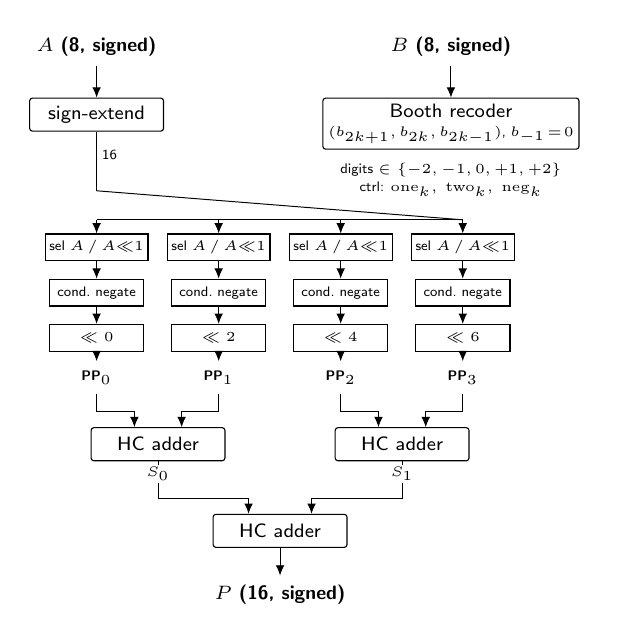
\begin{tikzpicture}[node distance=3mm]

% --- inputs ---
\node[io] (A) at (0,0) {$A$ (8, signed)};
\node[io] (B) at (4.5,0) {$B$ (8, signed)};

% --- sign extend / recoder ---
\node[blk, below=4mm of A, minimum width=17mm] (sx) {sign-extend};
\node[blk, below=4mm of B, minimum width=26mm] (rec)
      {Booth recoder\\[-1pt]{\tiny$(b_{2k+1},b_{2k},b_{2k-1})$, $b_{-1}\!=\!0$}};

\draw[wire] (A) -- (sx);
\draw[wire] (B) -- (rec);

% digit-set annotation
\node[font=\tiny\sffamily, right=1mm of rec.east, align=left, xshift=-1mm]
     {};
\node[font=\tiny\sffamily] at ($(rec.south)+(0,-2.6mm)$)
     {digits $\in\{-2,-1,0,+1,+2\}$};

% --- A bus rail feeding all 4 stages ---
\coordinate (rail) at ($(sx.south)+(0,-4mm)$);
\draw[plain] (sx) -- (rail);
\node[bw, right=0.4mm of rail, yshift=1.1mm] {16};

% --- four Booth PP stages ---
\foreach \i/\x/\sh in {0/0.0/0, 1/1.55/2, 2/3.1/4, 3/4.65/6} {
  \node[smallblk, minimum width=12mm] (sel\i) at (\x,-2.55)
        {sel $A\,/\,A{\ll}1$};
  \node[smallblk, minimum width=12mm, below=2.2mm of sel\i] (neg\i)
        {cond.\ negate};
  \node[smallblk, minimum width=12mm, below=2.2mm of neg\i] (sft\i)
        {$\ll\sh$};
  \draw[wire] (sel\i) -- (neg\i);
  \draw[wire] (neg\i) -- (sft\i);
  \node[font=\tiny\sffamily\bfseries, below=1.2mm of sft\i] (pp\i) {PP$_\i$};
  \draw[wire] (sft\i) -- (pp\i);
}

% rail into the four selects
\draw[plain] (rail) -- ($(rail)+(0,-0.35)$);
\coordinate (railL) at ($(rail)+(0,-0.35)$);
\draw[plain] (railL) -- (4.65,-2.20);
\draw[plain] (0,-2.20) -- (4.65,-2.20);
\foreach \i/\x in {0/0.0, 1/1.55, 2/3.1, 3/4.65} {
  \draw[wire] (\x,-2.20) -- (sel\i.north);
}

% recoder control lines into the stages (one/two/neg)
\node[font=\tiny\sffamily] at ($(rec.south)+(0,-5.0mm)$)
     {ctrl: $\mathrm{one}_k,\ \mathrm{two}_k,\ \mathrm{neg}_k$};

% --- adder tree ---
\node[blk, minimum width=17mm] (hc0) at (0.78,-5.05) {HC adder};
\node[blk, minimum width=17mm] (hc1) at (3.88,-5.05) {HC adder};
\node[blk, minimum width=17mm] (hc2) at (2.33,-6.15) {HC adder};

\draw[wire] (pp0) |- ($(hc0.north)+(-3mm,2mm)$) -- ($(hc0.north)+(-3mm,0)$);
\draw[wire] (pp1) |- ($(hc0.north)+(3mm,2mm)$)  -- ($(hc0.north)+(3mm,0)$);
\draw[wire] (pp2) |- ($(hc1.north)+(-3mm,2mm)$) -- ($(hc1.north)+(-3mm,0)$);
\draw[wire] (pp3) |- ($(hc1.north)+(3mm,2mm)$)  -- ($(hc1.north)+(3mm,0)$);

\draw[wire] (hc0.south) |- ($(hc2.north)+(-4mm,2mm)$) -- ($(hc2.north)+(-4mm,0)$);
\draw[wire] (hc1.south) |- ($(hc2.north)+(4mm,2mm)$)  -- ($(hc2.north)+(4mm,0)$);
\node[bw] at ($(hc0.south)+(0,-1.6mm)$) {$S_0$};
\node[bw] at ($(hc1.south)+(0,-1.6mm)$) {$S_1$};

% --- output ---
\node[io, below=3.5mm of hc2] (P) {$P$ (16, signed)};
\draw[wire] (hc2) -- (P);

\end{tikzpicture}
\caption{Datapath of the proposed signed radix-4 MRPM. The multiplier
operand is recoded two bits at a time into the digit set
$\{-2,-1,0,+1,+2\}$, yielding four partial products that are aligned by
hard-wired shifts and summed by a two-level parallel-prefix adder tree.}
\label{fig:mrpm}
\end{figure}

\subsection{Parallel-prefix addition}
\label{subsec:hc}

All additions --- both the partial-product accumulation of
Algorithm~\ref{alg:mrpm} and the filter summation of
Section~\ref{subsec:fold} --- are performed by a parallel-prefix adder.
Pre-processing forms the bitwise generate and propagate terms

\begin{equation}
g_i = a_i \cdot b_i, \qquad p_i = a_i \oplus b_i .
\label{eq:gp}
\end{equation}

\noindent A logarithmic-depth prefix network then combines these terms;
the carry into bit $i+1$ and the sum bit are

\begin{equation}
c_{i+1} = G_i + (P_i \cdot c_{\mathrm{in}}), \qquad
s_i = p_i \oplus c_i ,
\label{eq:sum}
\end{equation}

\noindent where $(G_i, P_i)$ denote the group generate and propagate
signals at the output of the prefix network.

Prefix topologies differ in how they trade depth against cell count and
fan-out. Kogge-Stone attains minimal depth ($\log_2 W$ for width $W$) at
the cost of the largest cell count and the heaviest routing. Brent-Kung
minimises cell count at roughly twice the depth. Sklansky attains
minimal depth with fewer cells, at the cost of fan-out that grows across
levels. Han-Carlson hybridises the Kogge-Stone and Brent-Kung schedules,
targeting depth $\approx \log_2 W + 1$ with substantially fewer cells.

Rather than assume a topology, we treat the choice as an empirical
question and synthesise all four within an otherwise identical filter
(Section~\ref{sec:results}). The four adders share a common port list
and are selected at compile time, so that any measured difference is
attributable to the prefix network alone.

\smallskip\noindent\textit{Disclosure on the realised networks.} The
adders are described behaviourally, and the structure committed to the
fabric is determined by the synthesiser rather than hand-instantiated at
the prefix-cell level. One consequence must be stated plainly: the
network we describe under a Han-Carlson schedule and the Kogge-Stone
network synthesise to the \emph{same} netlist on this fabric, and
therefore yield identical area, timing and power. We accordingly report
them as a single design point in Section~\ref{sec:results} rather than
as two, and we make no claim to have realised a distinct Han-Carlson
prefix structure. The comparison that follows is therefore between three
distinct synthesised prefix structures --- Kogge-Stone (equivalently, the
Han-Carlson-scheduled description), Brent-Kung and Sklansky --- all
derived from functionally equivalent descriptions and all verified to
produce identical arithmetic results (Section~\ref{sec:verif}).

\subsection{Symmetric-folded FIR filter}
\label{subsec:fold}

For a linear-phase FIR the coefficient set is symmetric,
$h[i] = h[N-1-i]$, as is the case for \eqref{eq:coeffs}. The direct-form
output

\begin{equation}
y[n] = \sum_{i=0}^{N-1} h[i]\, x[n-i]
\label{eq:direct}
\end{equation}

\noindent can therefore be regrouped by pairing each tap with its mirror
image:

\begin{equation}
y[n] = \sum_{i=0}^{N/2-1} h[i]\,\big(x[n-i] + x[n-(N-1-i)]\big).
\label{eq:folded}
\end{equation}

\noindent Equation~\eqref{eq:folded} is an algebraic identity, not an
approximation: it replaces $N$ multiplications by $N/2$ multiplications
and $N/2$ pre-additions, and its output is \emph{bit-identical} to
\eqref{eq:direct}. For $N = 8$ the multiplier count falls from eight to
four. Since the multiplier is by a wide margin the dominant consumer of
logic resources in the filter, and a pre-adder is far cheaper than a
multiplier, this is the principal area lever of the design.

Each pre-add sums two signed 8-bit samples and therefore requires one
guard bit, yielding a 9-bit signed operand; the multipliers are
correspondingly $9 \times 8$. The four products are summed by a
three-node Han-Carlson tree to a full-precision 20-bit signed output
(Section~\ref{sec:impl}). The resulting structure is shown in
Fig.~\ref{fig:fir}.

% ===================================================================
% FIGURE 2 : symmetric-folded 8-tap FIR (pre-adders VISIBLE)
% ===================================================================
\begin{figure}[t]
\centering
\resizebox{\columnwidth}{!}{%
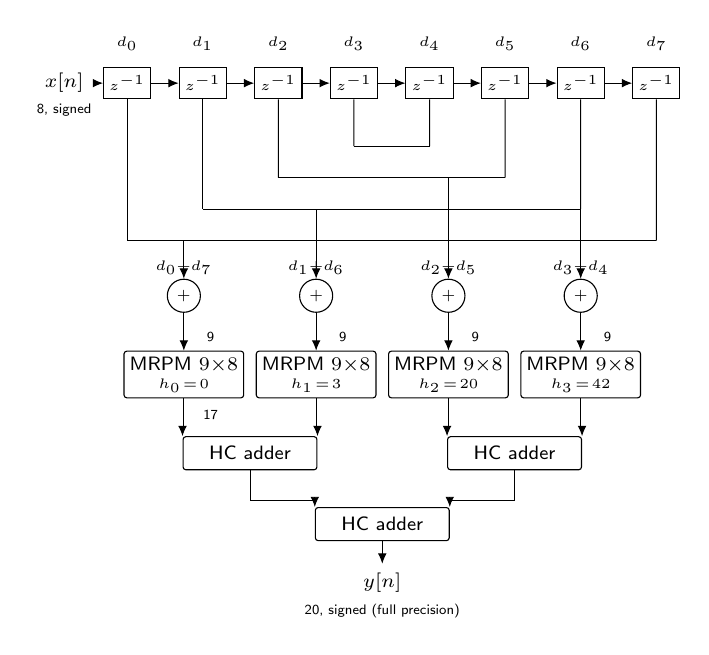
\begin{tikzpicture}[x=1mm, y=1mm]

% ---------- delay line (top) ----------
\node[io] (xin) at (-8,0) {$x[n]$};
\node[font=\tiny\sffamily] at (-8,-3.4) {8, signed};

\foreach \i in {0,...,7} {
  \pgfmathsetmacro\x{\i*9.6}
  \node[reg, minimum width=6mm] (d\i) at (\x,0) {$z^{-1}$};
  \node[font=\tiny\sffamily] at (\x,5.0) {$d_{\i}$};
}
\draw[wire] (xin.east) -- (d0.west);
\foreach \i [evaluate=\i as \j using int(\i+1)] in {0,...,6} {
  \draw[wire] (d\i.east) -- (d\j.west);
}

% ---------- routing bus rows (one row per mirror pair) ----------
% each pair gets its own horizontal lane so nothing overlaps
% lanes at y = -8, -12, -16, -20  (outermost pair uses the lowest lane)
\def\lanea{-20}   % d0 + d7  (outermost)
\def\laneb{-16}   % d1 + d6
\def\lanec{-12}   % d2 + d5
\def\laned{-8}    % d3 + d4  (innermost)

% pre-adder x-positions
\def\pxa{7.2}
\def\pxb{24.0}
\def\pxc{40.8}
\def\pxd{57.6}

% --- pair (d0,d7) -> pa0 ---
\draw[plain] (d0.south) -- (0,\lanea);
\draw[plain] (d7.south) -- (67.2,\lanea);
\draw[plain] (0,\lanea) -- (67.2,\lanea);

% --- pair (d1,d6) -> pa1 ---
\draw[plain] (d1.south) -- (9.6,\laneb);
\draw[plain] (d6.south) -- (57.6,\laneb);
\draw[plain] (9.6,\laneb) -- (57.6,\laneb);

% --- pair (d2,d5) -> pa2 ---
\draw[plain] (d2.south) -- (19.2,\lanec);
\draw[plain] (d5.south) -- (48.0,\lanec);
\draw[plain] (19.2,\lanec) -- (48.0,\lanec);

% --- pair (d3,d4) -> pa3 ---
\draw[plain] (d3.south) -- (28.8,\laned);
\draw[plain] (d4.south) -- (38.4,\laned);
\draw[plain] (28.8,\laned) -- (38.4,\laned);

% ---------- four PRE-ADDERS ----------
\node[addr] (pa0) at (\pxa,-27) {$+$};
\node[addr] (pa1) at (\pxb,-27) {$+$};
\node[addr] (pa2) at (\pxc,-27) {$+$};
\node[addr] (pa3) at (\pxd,-27) {$+$};

% drop each lane into its pre-adder
\draw[wire] (\pxa,\lanea) -- (pa0.north);
\draw[wire] (\pxb,\laneb) -- (pa1.north);
\draw[wire] (\pxc,\lanec) -- (pa2.north);
\draw[wire] (\pxd,\laned) -- (pa3.north);

% tick the lane taps so the pairing is unambiguous
\node[font=\tiny\sffamily] at (\pxa,-23.4) {$d_0{+}d_7$};
\node[font=\tiny\sffamily] at (\pxb,-23.4) {$d_1{+}d_6$};
\node[font=\tiny\sffamily] at (\pxc,-23.4) {$d_2{+}d_5$};
\node[font=\tiny\sffamily] at (\pxd,-23.4) {$d_3{+}d_4$};

% ---------- four multipliers (9x8, NOT 8x8) ----------
\node[blk, minimum width=15mm] (m0) at (\pxa,-37)
      {MRPM $9{\times}8$\\[-1.5pt]{\tiny$h_0\!=\!0$}};
\node[blk, minimum width=15mm] (m1) at (\pxb,-37)
      {MRPM $9{\times}8$\\[-1.5pt]{\tiny$h_1\!=\!3$}};
\node[blk, minimum width=15mm] (m2) at (\pxc,-37)
      {MRPM $9{\times}8$\\[-1.5pt]{\tiny$h_2\!=\!20$}};
\node[blk, minimum width=15mm] (m3) at (\pxd,-37)
      {MRPM $9{\times}8$\\[-1.5pt]{\tiny$h_3\!=\!42$}};

\foreach \i in {0,...,3} { \draw[wire] (pa\i.south) -- (m\i.north); }

% the 9-bit guard bit -- why the multipliers widen
\node[bw] at (\pxa+3.4,-32.2) {9};
\node[bw] at (\pxb+3.4,-32.2) {9};
\node[bw] at (\pxc+3.4,-32.2) {9};
\node[bw] at (\pxd+3.4,-32.2) {9};

% ---------- adder tree ----------
\node[blk, minimum width=17mm] (a0) at (15.6,-47) {HC adder};
\node[blk, minimum width=17mm] (a1) at (49.2,-47) {HC adder};
\node[blk, minimum width=17mm] (a2) at (32.4,-56) {HC adder};

\draw[wire] (m0.south) -- (\pxa,-44.0) -| (a0.north west);
\draw[wire] (m1.south) -- (\pxb,-44.0) -| (a0.north east);
\draw[wire] (m2.south) -- (\pxc,-44.0) -| (a1.north west);
\draw[wire] (m3.south) -- (\pxd,-44.0) -| (a1.north east);
\node[bw] at (\pxa+3.4,-42.2) {17};

\draw[wire] (a0.south) -- (15.6,-53.0) -| (a2.north west);
\draw[wire] (a1.south) -- (49.2,-53.0) -| (a2.north east);

% ---------- output ----------
\node[io] (yout) at (32.4,-63.5) {$y[n]$};
\node[font=\tiny\sffamily] at (32.4,-67.0) {20, signed (full precision)};
\draw[wire] (a2.south) -- (yout.north);

\end{tikzpicture}%
}
\caption{Symmetric-folded 8-tap linear-phase FIR. Mirror-image taps
($d_i$ with $d_{7-i}$) are pre-added before multiplication, halving the
multiplier count from eight to four with bit-identical output. Each
pre-adder widens the operand to nine bits, so the surviving multipliers
are $9{\times}8$; this is why the measured LUT4 saving is 35.7\% rather
than 50\%.}
\label{fig:fir}
\end{figure}

\subsection{Pipelining}
\label{subsec:pipe}

In its unpipelined form the folded filter presents a single
combinational path that traverses a complete multiplier and the full
summation tree, so the achievable clock frequency is bounded by the sum
of both. The datapath is therefore partitioned into four pipeline
stages, with register boundaries placed as follows:

\begin{itemize}
  \item \textbf{S1} --- the input delay line (already registered);
  \item \textbf{S2} --- within each multiplier, between Booth
  partial-product generation \eqref{eq:pp} and the accumulation tree;
  \item \textbf{S3} --- after the multipliers, at the inputs of the
  first level of the filter summation tree;
  \item \textbf{S4} --- after the first summation level, feeding the
  registered output.
\end{itemize}

The critical path is thereby reduced to approximately one adder level.
Latency rises from one cycle to four, while throughput remains one
sample per clock cycle in steady state; the functional output is
unchanged, which is confirmed in Section~\ref{sec:verif}.

% ===================================================================
\section{Implementation}
\label{sec:impl}

\subsection{Number formats and bit-growth}

The filter is realised in fixed-point arithmetic with the widths of
Table~\ref{tab:widths}. Input samples and coefficients are 8-bit signed
integers; the coefficients of \eqref{eq:coeffs} carry an implicit scale
factor of $2^7$, so the datapath output is the true filter response
scaled by $128$, and a deployed system applies a final arithmetic
right-shift of seven places.

Bit-growth is bounded as follows. Each mirror-pair pre-add of two
signed 8-bit samples requires one guard bit, giving a 9-bit operand.
Each $9 \times 8$ product is 17 bits. The worst-case magnitude of the
accumulated sum is bounded by

\begin{equation}
|y|_{\max} \;\le\; N \cdot |x|_{\max} \cdot |h|_{\max}
          \;=\; 8 \cdot 127 \cdot 128 \;=\; 130{,}048 ,
\label{eq:bitgrowth}
\end{equation}

\noindent which requires 18 bits in two's-complement representation. A
20-bit output is adopted, providing headroom
($2^{19} = 524{,}288$) and retaining full precision: no rounding,
truncation or saturation is applied anywhere in the datapath, so the
filter is numerically exact with respect to its integer specification.

\begin{table}[t]
\caption{Fixed-point widths and bit-growth}
\label{tab:widths}
\centering
\begin{tabular}{@{}lll@{}}
\toprule
\textbf{Quantity} & \textbf{Width} & \textbf{Rationale} \\
\midrule
Input $x$, coefficient $h$ & 8-bit signed & range $-128 \dots 127$ \\
Pre-add $x[n-i]+x[n-7+i]$  & 9-bit signed & one guard bit \\
Product ($9 \times 8$)     & 17-bit signed & --- \\
Output $y$                 & 20-bit signed & \eqref{eq:bitgrowth}; full precision \\
\bottomrule
\end{tabular}
\end{table}

\subsection{Design and verification flow}

The architecture is described in synthesisable Verilog. Functional
simulation and regression are performed with Icarus Verilog, with
waveform inspection in GTKWave. An independent golden model, written in
Python/NumPy, implements the radix-4 Booth recoding and the fixed-point
filter arithmetic; it is itself cross-checked against direct integer
convolution, so that the reference used to validate the RTL does not
share an implementation lineage with it. The complete regression suite
is driven by a single build target.

\subsection{Target device and DSP-disabled implementation flow}

The design targets the Gowin GW1NR-9C FPGA (8640 LUT4, 6480 flip-flops),
the device carried by the Sipeed Tang Nano 9K board and a substantially
lower-cost, lower-capacity part than the Xilinx Artix-7 used in
\cite{base}. Results are reported after synthesis and place-and-route;
the design was not downloaded to the device, and no claim of on-chip
execution is made.

One methodological point is essential to the validity of the area claim.
The GW1NR-9 fabric contains dedicated hardware multiplier (DSP)
resources, and a synthesiser will by default infer them from a
multiplication operator. Were this permitted, the reported LUT
utilisation would not reflect the cost of the proposed multiplier at
all, and the central claim of the paper --- that the architecture is an
area-efficient \emph{LUT-based} multiplier --- would be vacuous.
Synthesis is therefore constrained to logic-only mapping
(\texttt{syn\_multstyle = "logic"}), and the utilisation report is
required to show zero DSP blocks in use. This constraint is applied to
every configuration reported in Section~\ref{sec:results}, including
those used for the comparative adder sweep, so that all rows of that
comparison are measured on the same footing.

% ===================================================================
\section{Functional Verification}
\label{sec:verif}

Because the proposed design is an \emph{exact} multiplier --- in
deliberate contrast to the approximate architectures of
\cite{khurshid,approx2025} --- its correctness must be established
without residual error tolerance. Verification proceeds at three
levels.

\subsection{Exhaustive multiplier verification}

The signed radix-4 MRPM of Section~\ref{subsec:mult} is verified
\emph{exhaustively}. For an 8-bit signed multiplier the operand space
is finite and small: all $256 \times 256 = 65{,}536$ ordered pairs
$(a,b)$ with $a, b \in [-128, 127]$ are applied to the RTL and the
16-bit product is compared against the reference product $a \cdot b$.
The design produces \textbf{zero mismatches} across the entire operand
space. Exhaustive coverage is a stronger guarantee than the
best-case/worst-case/random-vector methodology usually reported for
multipliers of this width, since it admits no untested corner.

\subsection{Filter verification against an independent golden model}

The symmetric-folded 8-tap filter of Section~\ref{subsec:fold} is
verified against the Python golden model over a pseudo-random signed
input sequence. The RTL output matches the golden reference with
\textbf{zero mismatches}, confirming both the correctness of the
$9 \times 8$ multipliers and the exactness of the folding identity
\eqref{eq:folded}: the folded four-multiplier filter and the direct
eight-multiplier form produce bit-identical output, so the halving of
the multiplier count carries no numerical cost whatsoever.

\subsection{Pipeline and adder-variant equivalence}

Two further equivalence checks are performed. First, the four-stage
pipelined filter of Section~\ref{subsec:pipe} is compared against the
same golden reference with the output alignment adjusted for the
increased latency; it likewise produces \textbf{zero mismatches},
confirming that pipelining alters timing alone and not function.
Second, the filter is rebuilt with each prefix-adder description ---
Han-Carlson-scheduled, Kogge-Stone, Brent-Kung and Sklansky --- and each
configuration is re-verified; all pass with \textbf{zero mismatches}.
The adder sweep of Section~\ref{sec:results} therefore compares
\emph{functionally equivalent} implementations, so any difference
observed in area, delay or power is attributable to the prefix topology
alone.

\subsection{Summary}

Table~\ref{tab:verif} summarises the verification outcomes. Every
functional claim made in this paper is supported by simulation
evidence; the structural claims --- four partial products rather than
eight iterations, four multipliers rather than eight, signed operand
support --- follow directly from the architecture and are independent
of synthesis.

\begin{table}[t]
\caption{Functional verification results}
\label{tab:verif}
\centering
\begin{tabular}{@{}llc@{}}
\toprule
\textbf{Design under test} & \textbf{Method} & \textbf{Mismatches} \\
\midrule
Signed radix-4 MRPM ($8\times8$) & exhaustive, 65{,}536 pairs & 0 \\
Folded 8-tap FIR                 & golden model               & 0 \\
Pipelined folded FIR             & golden model, latency-4    & 0 \\
FIR, Han-Carlson-scheduled adder & golden model               & 0 \\
FIR, Kogge-Stone adder           & golden model               & 0 \\
FIR, Brent-Kung adder            & golden model               & 0 \\
FIR, Sklansky adder              & golden model               & 0 \\
\bottomrule
\end{tabular}
\end{table}

\subsection{Structural comparison}

Independently of synthesis, the proposed architecture differs
structurally from \cite{base} as summarised in Table~\ref{tab:struct}.
These figures follow from the algorithm and the filter topology and
require no measurement.

\begin{table}[t]
\caption{Structural comparison with the base architecture}
\label{tab:struct}
\centering
\begin{tabular}{@{}lccc@{}}
\toprule
\textbf{Design} & \textbf{Mult.\ in FIR} & \textbf{PPs / iter.} &
\textbf{Signed} \\
\midrule
Base MRPM \cite{base}      & 8                   & $\sim$8 iterations & No  \\
This work, direct          & 8                   & 4 partial products & Yes \\
This work, folded          & \textbf{4}          & 4 partial products & Yes \\
\bottomrule
\end{tabular}
\end{table}

% ===================================================================
\section{Synthesis Results and Discussion}
\label{sec:results}

All configurations were synthesised and placed-and-routed for the Gowin
GW1NR-9C, the device carried by the Sipeed Tang Nano 9K board. In every
run, DSP inference was disabled and the utilisation report was checked to
confirm that \textbf{zero DSP blocks} were used; the reported LUT4
figures therefore reflect the true cost of realising the arithmetic in
general-purpose logic. All figures below are read directly from Gowin
post-place-and-route utilisation, timing and power reports. We report
implementation results at the place-and-route level; on-chip execution of
the filter is outside the scope of this study and is noted as future
work.

\subsection{Effect of symmetric folding}

Table~\ref{tab:util} compares the direct 8-multiplier filter against the
symmetric-folded 4-multiplier filter. Folding reduces LUT4 utilisation
from 345 to 222, a saving of \textbf{35.7\%}, while flip-flop count,
power and $F_{\max}$ are essentially unchanged. The output is
bit-identical (Section~\ref{sec:verif}), so this saving is obtained at
no numerical cost whatsoever.

It is worth being precise about why the saving is 35.7\% and not the
50\% that a naive reading of ``eight multipliers become four'' would
suggest. Two effects erode the ideal figure. First, folding widens the
multiplicand: the pre-add of two signed 8-bit samples produces a 9-bit
operand, so the four surviving multipliers are $9 \times 8$ rather than
$8 \times 8$, and each is individually more expensive than the units it
replaces. Second, the four mirror-pair pre-adders are new logic that did
not exist in the direct form. The realised saving is thus

\begin{equation}
8 \cdot M_{8\times8} \;\longrightarrow\;
4 \cdot M_{9\times8} \;+\; 4 \cdot A_{9},
\label{eq:foldcost}
\end{equation}

\noindent rather than a clean halving. That 35.7\% survives both effects
confirms that the multiplier remains the dominant resource and that
trading multipliers for pre-adders is strongly favourable.

\begin{table}[t]
\caption{Resource utilisation and timing (Tang Nano 9K, GW1NR-9C, DSP disabled)}
\label{tab:util}
\centering
\begin{tabular}{@{}lccccc@{}}
\toprule
\textbf{Configuration} & \textbf{LUT4} & \textbf{FF} & \textbf{DSP} &
\textbf{$F_{\max}$} & \textbf{Power} \\
 & & & & \textbf{(MHz)} & \textbf{(mW)} \\
\midrule
Direct FIR (8 mult.)    & 345 & 44  & 0 & 42.858 & 2.582 \\
Folded FIR (4 mult.)    & \textbf{222} & 44  & 0 & 42.956 & 2.595 \\
Folded + pipelined      & 324 & 159 & 0 & \textbf{66.471} & 2.639 \\
\bottomrule
\end{tabular}
\end{table}

\subsection{Effect of pipelining}

The four-stage pipeline raises $F_{\max}$ from 42.96~MHz to 66.47~MHz, a
speed-up of $\mathbf{1.55\times}$, at a cost of 115 additional
flip-flops (44 to 159) and 102 additional LUT4 (222 to 324), with
latency rising from one cycle to four and throughput unchanged at one
sample per cycle. Dynamic power rises only marginally, from 2.595~mW to
2.639~mW. The pipelined design remains smaller than the unpipelined
\emph{direct} filter (324 versus 345 LUT4) while running 55\% faster,
so folding and pipelining together dominate the direct form on both
axes simultaneously.

\subsection{Prefix-adder comparison}

Table~\ref{tab:adders} reports the folded filter rebuilt around each
prefix topology. As disclosed in Section~\ref{subsec:hc}, the
Han-Carlson-scheduled description and the Kogge-Stone network synthesise
to the same netlist and are therefore reported as a single point.

The result is, in our view, the most useful finding of the sweep, and it
is a largely negative one: \emph{at 8-bit datapath width the choice of
prefix adder scarcely matters}. Across three distinct synthesised
structures the spread is 222 to 238 LUT4 (7\%) and 41.76 to 44.96~MHz
(7.6\%), with dynamic power varying by less than 0.2\%. Sklansky is the
fastest by 4.7\% but pays 16 additional LUT4 for it; Brent-Kung offers
no advantage on this fabric, being marginally both larger and slower
than Kogge-Stone. Flip-flop count is identical throughout.

This has a direct bearing on the architecture of \cite{base}. At the
widths characteristic of a biomedical datapath, the depth advantage of a
minimum-depth prefix network amounts to roughly one logic level, and its
effect is small compared with the structural levers examined above:
folding alone returns 35.7\% of the LUT4 budget, and pipelining alone
returns $1.55\times$ in frequency, whereas the entire span of the adder
sweep is 7\%. Effort spent selecting among prefix topologies at this
width is, on this evidence, effort misdirected.

\begin{table}[t]
\caption{Prefix-adder comparison (folded 8-tap FIR, identical otherwise)}
\label{tab:adders}
\centering
\begin{tabular}{@{}lccccc@{}}
\toprule
\textbf{Prefix adder} & \textbf{LUT4} & \textbf{FF} &
\textbf{$F_{\max}$} & \textbf{Power} & \textbf{Func.} \\
 & & & \textbf{(MHz)} & \textbf{(mW)} & \\
\midrule
Kogge-Stone$^{\dagger}$ & \textbf{222} & 44 & 42.956 & \textbf{2.595} & PASS \\
Brent-Kung              & 223 & 44 & 41.762 & 2.595 & PASS \\
Sklansky                & 238 & 44 & \textbf{44.955} & 2.599 & PASS \\
\bottomrule
\multicolumn{6}{@{}p{0.95\columnwidth}@{}}{\footnotesize $^{\dagger}$The
Han-Carlson-scheduled description synthesises to this same netlist and is
therefore not reported as a separate point (Section~\ref{subsec:hc}).}
\end{tabular}
\end{table}

\subsection{Comparison with the base architecture}
\label{subsec:basecmp}

Table~\ref{tab:base} places this work alongside the figures reported in
\cite{base}. \textbf{These rows are not like-for-like, and we do not
present them as such.} Four differences must be held in mind.

\begin{enumerate}
  \item \textbf{Different units of measurement.} Reference \cite{base}
  characterises a \emph{standalone unsigned multiplier}; the figures
  reported here characterise a \emph{complete signed 8-tap FIR filter},
  which contains four multipliers together with a delay line,
  pre-adders and a summation tree. A LUT count for one is not
  commensurable with a LUT count for the other.

  \item \textbf{Different fabrics.} The base design targets a Xilinx
  Artix-7 (Nexys A7), whose 6-input LUTs differ structurally from the
  LUT4 primitives of the Gowin GW1NR-9C. Raw LUT counts do not transfer
  between the two.

  \item \textbf{Different power methodology.} The 1.136~W reported in
  \cite{base} and the 2.595~mW reported here differ by three orders of
  magnitude, which is not plausibly a design difference. The two figures
  are evidently obtained under different power-estimation assumptions,
  and \emph{we therefore make no power claim of any kind against
  \cite{base}}.

  \item \textbf{Different frequency semantics.} The 0.714~MHz of
  \cite{base} is consistent with the result rate of an iterative,
  multi-cycle multiplier, whereas the 42.96/66.47~MHz reported here is
  the maximum clock frequency of a parallel datapath. The gap reflects
  an architectural difference --- iterative versus parallel evaluation
  --- and not superior timing closure of the same structure.
\end{enumerate}

\subsection{The multiplier in isolation: an explicit area--time trade}
\label{subsec:standalone}

The filter-level figures above do not answer the question a reader will
ask directly: how large is the proposed multiplier on its own? We
therefore synthesised the standalone $8 \times 8$ signed radix-4 MRPM
through the same flow. It occupies \textbf{170 LUT4}, with zero
registers, zero DSP blocks and 32 I/O ports, and is purely
combinational.

We state the comparison plainly. The unsigned iterative multiplier of
\cite{base} occupies 68 LUT; the proposed signed parallel multiplier
occupies 170 LUT4. \emph{At the level of the multiplier alone, the
proposed design is the larger of the two}, and we make no claim to the
contrary. Part of the difference is an artefact of the fabric --- the
6-input LUTs of the Artix-7 absorb more logic per cell than the LUT4
primitives of the GW1NR-9C, so the raw ratio overstates the true gap ---
but the direction of the difference is not in doubt, and it is a direct
and intended consequence of two design decisions.

The first is signedness. Two's-complement operation requires sign
extension through every partial product and a conditional negation
(inversion and increment) at each Booth digit, none of which an unsigned
datapath pays for. The second, and larger, is parallelism. The proposed
multiplier instantiates four partial-product generators and a summation
tree \emph{in space}; the design of \cite{base} instantiates a single
adder and reuses it \emph{in time} across approximately eight
iterations. Spatial evaluation costs area by construction. This is the
classical area--time trade-off, and the corresponding entry in the base
design's own results is its 0.714~MHz result rate: its compactness is
purchased with sequential cycles. Comparing the area of an iterative
multiplier with that of a parallel one, without quoting the throughput
each achieves, is not a meaningful comparison.

\smallskip\noindent\textit{Why this does not undermine the area claim.}
The standalone figure is, in any case, not the figure on which this
paper's area efficiency rests. Two observations follow. First, four
standalone multipliers would account for roughly $4 \times 170 = 680$
LUT4, yet the complete folded filter --- multipliers, delay line,
pre-adders and summation tree together --- occupies 222 LUT4. The
difference is constant-coefficient specialisation: within the filter each
multiplier's second operand is a fixed coefficient
(\eqref{eq:coeffs}), and the synthesiser collapses the corresponding
logic aggressively, to the point of eliminating the $h_0 = 0$ multiplier
altogether. A general-purpose multiplier and a coefficient-specialised
one are therefore different objects, and the standalone number is a poor
predictor of the deployed one.

Second, and decisively, the claim of area efficiency advanced in this
paper is made against a like-for-like baseline rather than across
fabrics: the same filter, on the same device, through the same
toolchain, falls from 345 to 222 LUT4 --- a reduction of 35.7\% --- with
bit-identical output (Table~\ref{tab:util}). That measurement holds
regardless of how the standalone multiplier compares with \cite{base},
and it is the measurement on which the title's claim depends. What the
present subsection establishes is the price of the architectural change:
a larger multiplier, bought deliberately, in exchange for signed
operation and a throughput roughly two orders of magnitude higher, and
recovered at the filter level by folding.

The architectural comparison is summarised in Table~\ref{tab:base}.

\begin{table}[t]
\caption{Architectural comparison with the base design \cite{base}}
\label{tab:base}
\centering
\begin{tabular}{@{}lcc@{}}
\toprule
 & \textbf{Base \cite{base}} & \textbf{This work} \\
\midrule
Standalone mult.\ area & 68 LUT (6-LUT)  & 170 LUT4 \\
Complete FIR area    & not reported      & \textbf{222 LUT4} \\
Multiplier rate      & 0.714 MHz (iter.) & \textbf{single-cycle} \\
Filter $F_{\max}$    & not reported      & \textbf{42.96 / 66.47 MHz} \\
Operands             & unsigned          & \textbf{signed} \\
Multiplier evaluation & $\sim$8 iterations & \textbf{4 parallel PPs} \\
Multipliers in FIR   & 8                 & \textbf{4} (folded) \\
Pipelining           & ---               & \textbf{4-stage} \\
Adder study          & single (KS)       & \textbf{3 topologies swept} \\
Target fabric        & Artix-7 (Nexys A7) & Gowin GW1NR-9C \\
DSP blocks           & ---               & \textbf{0 (enforced)} \\
Exactness            & exact             & exact (exhaustive) \\
\bottomrule
\end{tabular}
\end{table}

\subsection{Discussion}

Three observations follow from the data. First, the structural levers
dominate: folding returns 35.7\% of the logic budget and pipelining
returns $1.55\times$ in frequency, while the entire prefix-adder sweep
spans 7\%. An architecture that accelerates the adder inside an
iterative loop, as in \cite{base}, is therefore optimising a term that
is not the binding one; the partial-product count and the filter
structure are.

Second, the folded design is strictly better than the direct design on
every axis measured --- 35.7\% fewer LUT4, identical flip-flops,
marginally higher $F_{\max}$, and bit-identical output --- so there is no
trade-off to negotiate. Folding should be regarded as the default for
any linear-phase FIR.

Third, the pipelined folded design is smaller than the \emph{direct}
design (324 versus 345 LUT4) while running 1.55$\times$ faster than the
folded design, at the price of three additional cycles of latency. For a
front-end ECG filter sampling at 250~Hz, a latency of four clock cycles
at tens of megahertz is entirely negligible, so the pipelined
configuration is the appropriate operating point for deployment.

\section{Conclusion}
\label{sec:concl}

This paper has presented an area-efficient, exact, signed multiplier
architecture for biomedical FIR filtering, extending the Modified
Russian Peasant Multiplier of \cite{base}. Radix-4 modified-Booth
recoding replaces approximately eight sequential iterations with four
partial products evaluated in parallel, and adds native
two's-complement support. Exploiting the linear-phase symmetry of the
coefficient set folds the 8-tap filter onto four multipliers rather than
eight, reducing LUT4 utilisation by 35.7\% (345 to 222) with provably
bit-identical output. A four-stage pipeline raises the maximum clock
frequency by $1.55\times$ (42.96~MHz to 66.47~MHz) for 115 additional
flip-flops, leaving the pipelined folded filter both smaller and
substantially faster than the unfolded, unpipelined design.

A comparative sweep of three synthesised prefix-adder topologies
returned a largely negative but instructive result: at 8-bit datapath
width the choice of prefix network spans only 7\% in area and 7.6\% in
frequency, an order of magnitude less than the structural levers. This
suggests that, for datapaths of the width typical in biomedical signal
processing, effort is better spent on the partial-product count and the
filter topology than on the adder --- and, by implication, that the
adder-centric optimisation pursued in \cite{base} addresses a term that
is not the binding constraint.

We also report, without qualification, the price of the architecture. In
isolation the proposed signed parallel multiplier occupies 170 LUT4
against the 68 LUT of the unsigned iterative design of \cite{base}: at
the level of the multiplier alone it is the larger of the two. That cost
buys signed operation and single-cycle evaluation in place of an
eight-iteration sequential loop, and it is recovered at the filter level,
where coefficient specialisation and symmetric folding bring the complete
filter to 222 LUT4.

Correctness was established without residual error tolerance: the
multiplier is verified exhaustively over all $65{,}536$ signed operand
pairs with zero mismatches, and every filter configuration --- folded,
pipelined, and with each prefix adder --- matches an independent golden
model exactly. All results were obtained with DSP inference disabled and
zero DSP blocks confirmed, so the reported area reflects genuine
logic-fabric cost.

\smallskip\noindent\textbf{Future work.} Two extensions follow
directly. First, the results reported here are obtained at the
place-and-route level; downloading the design to the device and
exercising it on-chip would confirm the timing closure empirically.
Second, the filter should be integrated into a complete acquisition
chain and evaluated on real electrocardiogram and electroencephalogram
recordings, so that denoising performance can be quantified on clinical
signal-quality metrics rather than on synthetic vectors alone. A third
direction, suggested by Section~\ref{subsec:standalone}, is to quantify
the area--time curve directly, by synthesising radix-2 and radix-8
variants of the multiplier alongside the radix-4 design reported here.

\begin{thebibliography}{00}

\bibitem{base}
G.~S. Subramanian~V., D.~S. T.N., and Aditya~S., ``A low cost
area-efficient modified Russian peasant multiplier (MRPM) for
biomedical applications,'' \emph{Integration, the VLSI Journal},
vol.~104, art.~102474, 2025.

\bibitem{sharma}
M.~Sharma and S.~K. Singh, ``New technique based Peasant multiplication
for efficient signal processing applications,'' \emph{Indonesian J.
Electr. Eng. Comput. Sci.}, vol.~8, no.~3, p.~726, 2017.

\bibitem{lotfabadi}
S.~S. Lotfabadi, A.~Ye, and S.~Krishnan, ``Measuring the power
efficiency of sub-threshold FPGAs for implementing portable biomedical
applications,'' \emph{Microprocess. Microsyst.}, vol.~36, no.~3,
pp.~151--158, 2012.

\bibitem{ajay}
A.~Ajay and R.~M. Lourde, ``VLSI implementation of an improved
multiplier for FFT computation in biomedical applications,'' in
\emph{Proc. IEEE Comput. Soc. Annu. Symp. VLSI}, 2015, pp.~68--73.

\bibitem{phuse}
A.~Phuse and P.~Tasgaonkar, ``Design and implementation of different
multiplier techniques and efficient MAC unit on FPGA,'' in \emph{Proc.
Int. Conf. Signal Inf. Process. (ICONSIP)}, 2022, pp.~1--5.

\bibitem{prabhu}
A.~S. Prabhu and V.~Elakya, ``Design of modified low power Booth
multiplier,'' in \emph{Proc. Int. Conf. Comput. Commun. Appl.}, 2012,
pp.~1--6.

\bibitem{kumar}
C.~U. Kumar and B.~J. Rabi, ``Design and implementation of modified
Russian Peasant multiplier using MSQRTCSLA based FIR filter,''
\emph{Indian J. Sci. Technol.}, vol.~9, no.~7, 2016.

\bibitem{gokhale}
G.~R. Gokhale and P.~D. Bahirgonde, ``Design of Vedic multiplier using
area-efficient carry select adder,'' in \emph{Proc. Int. Conf. Adv.
Comput. Commun. Informat. (ICACCI)}, 2015, pp.~576--581.

\bibitem{bansal}
Y.~Bansal, C.~Madhu, and P.~Kaur, ``High speed Vedic multiplier
designs---a review,'' in \emph{Proc. Recent Adv. Eng. Comput. Sci.
(RAECS)}, 2014, pp.~1--6.

\bibitem{rao}
E.~J. Rao, T.~Ramanjaneyulu, and K.~J. Kumar, ``Advanced multiplier
design and implementation using Han-Carlson adder,'' in \emph{Proc.
Int. Conf. Intell. Innov. Comput. Appl. (ICONIC)}, 2018, pp.~1--5.

\bibitem{dhole}
S.~Dhole, S.~Shembalkar, T.~Yadav, and P.~Thakre, ``Design and FPGA
implementation of 4$\times$4 Vedic multiplier using different
architectures,'' \emph{Int. J. Eng. Res. Technol.}, vol.~6, no.~4, 2017.

\bibitem{penchalaiah}
U.~Penchalaiah and S.~K. VG, ``Design of high-speed and energy-efficient
parallel prefix Kogge-Stone adder,'' in \emph{Proc. IEEE Int. Conf.
Syst. Comput. Autom. Netw. (ICSCAN)}, 2018, pp.~1--7.

\bibitem{raju}
A.~Raju and S.~K. Sa, ``Design and performance analysis of multipliers
using Kogge-Stone adder,'' in \emph{Proc. Int. Conf. Appl. Theor.
Comput. Commun. Technol. (iCATccT)}, 2017, pp.~94--99.

\bibitem{gunasekaran}
K.~Gunasekaran and M.~Manikandan, ``High speed reconfigurable FIR filter
using Russian Peasant multiplier with Sklansky adder,'' \emph{Res. J.
Appl. Sci. Eng. Technol.}, vol.~8, no.~24, pp.~2451--2456, 2014.

\bibitem{paz}
P.~Paz and M.~Garrido, ``Efficient implementation of complex multipliers
on FPGAs using DSP slices,'' \emph{J. Signal Process. Syst.}, vol.~95,
no.~4, pp.~543--550, 2023.

\bibitem{khurshid}
B.~Khurshid, ``FPGA-based resource-optimal approximate multiplier for
error-resilient applications,'' \emph{Int. J. Circuit Theory Appl.},
2024.

\bibitem{approx2025}
A.~K, S.~Sushma, and V.~S. Teja, ``Improving error resilience in
FPGA-based multi-level approximate multipliers using modified full
adders,'' in \emph{Proc. Int. Conf. Device Intell. Comput. Commun.
Technol. (DICCT)}, 2025, pp.~153--158.

\bibitem{anjana}
R.~Anjana, B.~Abishna, M.~S. Harshitha, E.~Abhishek, V.~Ravichandra, and
M.~S. Suma, ``Implementation of Vedic multiplier using Kogge-Stone
adder,'' in \emph{Proc. Int. Conf. Embedded Syst. (ICES)}, 2014,
pp.~28--31.

\bibitem{abed}
S.~Abed, B.~J. Mohd, Z.~Al-bayati, and S.~Alouneh, ``Low power Wallace
multiplier design based on wide counters,'' \emph{Int. J. Circuit Theory
Appl.}, vol.~40, no.~11, pp.~1175--1185, 2012.

\bibitem{badawi}
A.~Badawi, A.~Alqarni, A.~Aljuffri, M.~S. BenSaleh, A.~M. Obeid, and
S.~M. Qasim, ``FPGA realization and performance evaluation of
fixed-width modified Baugh-Wooley multiplier,'' in \emph{Proc. Int.
Conf. Technol. Adv. Electr. Electron. Comput. Eng. (TAEECE)}, 2015,
pp.~155--158.

\bibitem{tangnano}
Sipeed, ``Tang Nano 9K FPGA development board (Gowin GW1NR-9)
datasheet,'' 2023. [Online]. Available: \url{https://wiki.sipeed.com/}

\end{thebibliography}

\end{document}
